\documentclass[11pt,a4paper,]{article}
\usepackage{lmodern}

\usepackage{amssymb,amsmath}
\usepackage{ifxetex,ifluatex}
\usepackage{fixltx2e} % provides \textsubscript
\ifnum 0\ifxetex 1\fi\ifluatex 1\fi=0 % if pdftex
  \usepackage[T1]{fontenc}
  \usepackage[utf8]{inputenc}
\else % if luatex or xelatex
  \usepackage{unicode-math}
  \defaultfontfeatures{Ligatures=TeX,Scale=MatchLowercase}
\fi
% use upquote if available, for straight quotes in verbatim environments
\IfFileExists{upquote.sty}{\usepackage{upquote}}{}
% use microtype if available
\IfFileExists{microtype.sty}{%
\usepackage[]{microtype}
\UseMicrotypeSet[protrusion]{basicmath} % disable protrusion for tt fonts
}{}
\PassOptionsToPackage{hyphens}{url} % url is loaded by hyperref
\usepackage[unicode=true]{hyperref}
\hypersetup{
            pdftitle={Assignment3\_Group6},
            pdfborder={0 0 0},
            breaklinks=true}
\urlstyle{same}  % don't use monospace font for urls
\usepackage{geometry}
\geometry{a4paper, centering, text={16cm,24cm}}
\usepackage[style=authoryear-comp,]{biblatex}
\addbibresource{references.bib}
\usepackage{longtable,booktabs}
% Fix footnotes in tables (requires footnote package)
\IfFileExists{footnote.sty}{\usepackage{footnote}\makesavenoteenv{long table}}{}
\IfFileExists{parskip.sty}{%
\usepackage{parskip}
}{% else
\setlength{\parindent}{0pt}
\setlength{\parskip}{6pt plus 2pt minus 1pt}
}
\setlength{\emergencystretch}{3em}  % prevent overfull lines
\providecommand{\tightlist}{%
  \setlength{\itemsep}{0pt}\setlength{\parskip}{0pt}}
\setcounter{secnumdepth}{5}

% set default figure placement to htbp
\makeatletter
\def\fps@figure{htbp}
\makeatother


\title{Assignment3\_Group6}

%% MONASH STUFF

%% CAPTIONS
\RequirePackage{caption}
\DeclareCaptionStyle{italic}[justification=centering]
 {labelfont={bf},textfont={it},labelsep=colon}
\captionsetup[figure]{style=italic,format=hang,singlelinecheck=true}
\captionsetup[table]{style=italic,format=hang,singlelinecheck=true}


%% FONT
\RequirePackage{bera}
\RequirePackage[charter,expert,sfscaled]{mathdesign}
\RequirePackage{fontawesome}

%% HEADERS AND FOOTERS
\RequirePackage{fancyhdr}
\pagestyle{fancy}
\rfoot{\Large\sffamily\raisebox{-0.1cm}{\textbf{\thepage}}}
\makeatletter
\lhead{\textsf{\expandafter{\@title}}}
\makeatother
\rhead{}
\cfoot{}
\setlength{\headheight}{15pt}
\renewcommand{\headrulewidth}{0.4pt}
\renewcommand{\footrulewidth}{0.4pt}
\fancypagestyle{plain}{%
\fancyhf{} % clear all header and footer fields
\fancyfoot[C]{\sffamily\thepage} % except the center
\renewcommand{\headrulewidth}{0pt}
\renewcommand{\footrulewidth}{0pt}}

%% MATHS
\RequirePackage{bm,amsmath}
\allowdisplaybreaks

%% GRAPHICS
\RequirePackage{graphicx}
\setcounter{topnumber}{2}
\setcounter{bottomnumber}{2}
\setcounter{totalnumber}{4}
\renewcommand{\topfraction}{0.85}
\renewcommand{\bottomfraction}{0.85}
\renewcommand{\textfraction}{0.15}
\renewcommand{\floatpagefraction}{0.8}


%\RequirePackage[section]{placeins}

%% SECTION TITLES


%% SECTION TITLES (NEW: Changing sections and subsections color)
\RequirePackage[compact,sf,bf]{titlesec}
\titleformat*{\section}{\Large\sf\bfseries\color[rgb]{0.8, 0.7, 0.1 }}
\titleformat*{\subsection}{\large\sf\bfseries\color[rgb]{0.8, 0.7, 0.1 }}
\titleformat*{\subsubsection}{\sf\bfseries\color[rgb]{0.8, 0.7, 0.1 }}
\titlespacing{\section}{0pt}{2ex}{.5ex}
\titlespacing{\subsection}{0pt}{1.5ex}{0ex}
\titlespacing{\subsubsection}{0pt}{.5ex}{0ex}


%% TITLE PAGE
\def\Date{\number\day}
\def\Month{\ifcase\month\or
 January\or February\or March\or April\or May\or June\or
 July\or August\or September\or October\or November\or December\fi}
\def\Year{\number\year}

%% LINE AND PAGE BREAKING
\sloppy
\clubpenalty = 10000
\widowpenalty = 10000
\brokenpenalty = 10000
\RequirePackage{microtype}

%% PARAGRAPH BREAKS
\setlength{\parskip}{1.4ex}
\setlength{\parindent}{0em}

%% HYPERLINKS
\RequirePackage{xcolor} % Needed for links
\definecolor{darkblue}{rgb}{0,0,.6}
\RequirePackage{url}

\makeatletter
\@ifpackageloaded{hyperref}{}{\RequirePackage{hyperref}}
\makeatother
\hypersetup{
     citecolor=0 0 0,
     breaklinks=true,
     bookmarksopen=true,
     bookmarksnumbered=true,
     linkcolor=darkblue,
     urlcolor=blue,
     citecolor=darkblue,
     colorlinks=true}

\usepackage[showonlyrefs]{mathtools}
\usepackage[no-weekday]{eukdate}

%% BIBLIOGRAPHY

\makeatletter
\@ifpackageloaded{biblatex}{}{\usepackage[style=authoryear-comp, backend=biber, natbib=true]{biblatex}}
\makeatother
\ExecuteBibliographyOptions{bibencoding=utf8,minnames=1,maxnames=3, maxbibnames=99,dashed=false,terseinits=true,giveninits=true,uniquename=false,uniquelist=false,doi=false, isbn=false,url=true,sortcites=false}

\DeclareFieldFormat{url}{\texttt{\url{#1}}}
\DeclareFieldFormat[article]{pages}{#1}
\DeclareFieldFormat[inproceedings]{pages}{\lowercase{pp.}#1}
\DeclareFieldFormat[incollection]{pages}{\lowercase{pp.}#1}
\DeclareFieldFormat[article]{volume}{\mkbibbold{#1}}
\DeclareFieldFormat[article]{number}{\mkbibparens{#1}}
\DeclareFieldFormat[article]{title}{\MakeCapital{#1}}
\DeclareFieldFormat[article]{url}{}
%\DeclareFieldFormat[book]{url}{}
%\DeclareFieldFormat[inbook]{url}{}
%\DeclareFieldFormat[incollection]{url}{}
%\DeclareFieldFormat[inproceedings]{url}{}
\DeclareFieldFormat[inproceedings]{title}{#1}
\DeclareFieldFormat{shorthandwidth}{#1}
%\DeclareFieldFormat{extrayear}{}
% No dot before number of articles
\usepackage{xpatch}
\xpatchbibmacro{volume+number+eid}{\setunit*{\adddot}}{}{}{}
% Remove In: for an article.
\renewbibmacro{in:}{%
  \ifentrytype{article}{}{%
  \printtext{\bibstring{in}\intitlepunct}}}

\AtEveryBibitem{\clearfield{month}}
\AtEveryCitekey{\clearfield{month}}

\makeatletter
\DeclareDelimFormat[cbx@textcite]{nameyeardelim}{\addspace}
\makeatother

\author{\sf\Large\textbf{ Chatpisut Makornkhan}\\ {\sf\large Master of Business Analytics\\[0.5cm]} \sf\Large\textbf{ BINGYU YANG}\\ {\sf\large Master of Business Analytics\\[0.5cm]} \sf\Large\textbf{ Phuong Trinh}\\ {\sf\large Master of Business Analytics\\[0.5cm]}}

\date{\sf\Date~\Month~\Year}
\makeatletter
\lfoot{\sf Makornkhan, YANG, Trinh: \@date}
\makeatother


%%%% PAGE STYLE FOR FRONT PAGE OF REPORTS

\makeatletter
\def\organization#1{\gdef\@organization{#1}}
\def\telephone#1{\gdef\@telephone{#1}}
\def\email#1{\gdef\@email{#1}}
\makeatother
  \organization{Monash University}

  \def\name{Faculty of \newline Business \&\newline Economics}

  \telephone{(03) 9905 2478}

  \email{questions@company.com}                 %NEW: New email addresss

\def\webaddress{\url{http://company.com/stats/consulting/}} %NEW: URl
\def\abn{12 377 614 630}                                    % NEW: ABN
\def\logo{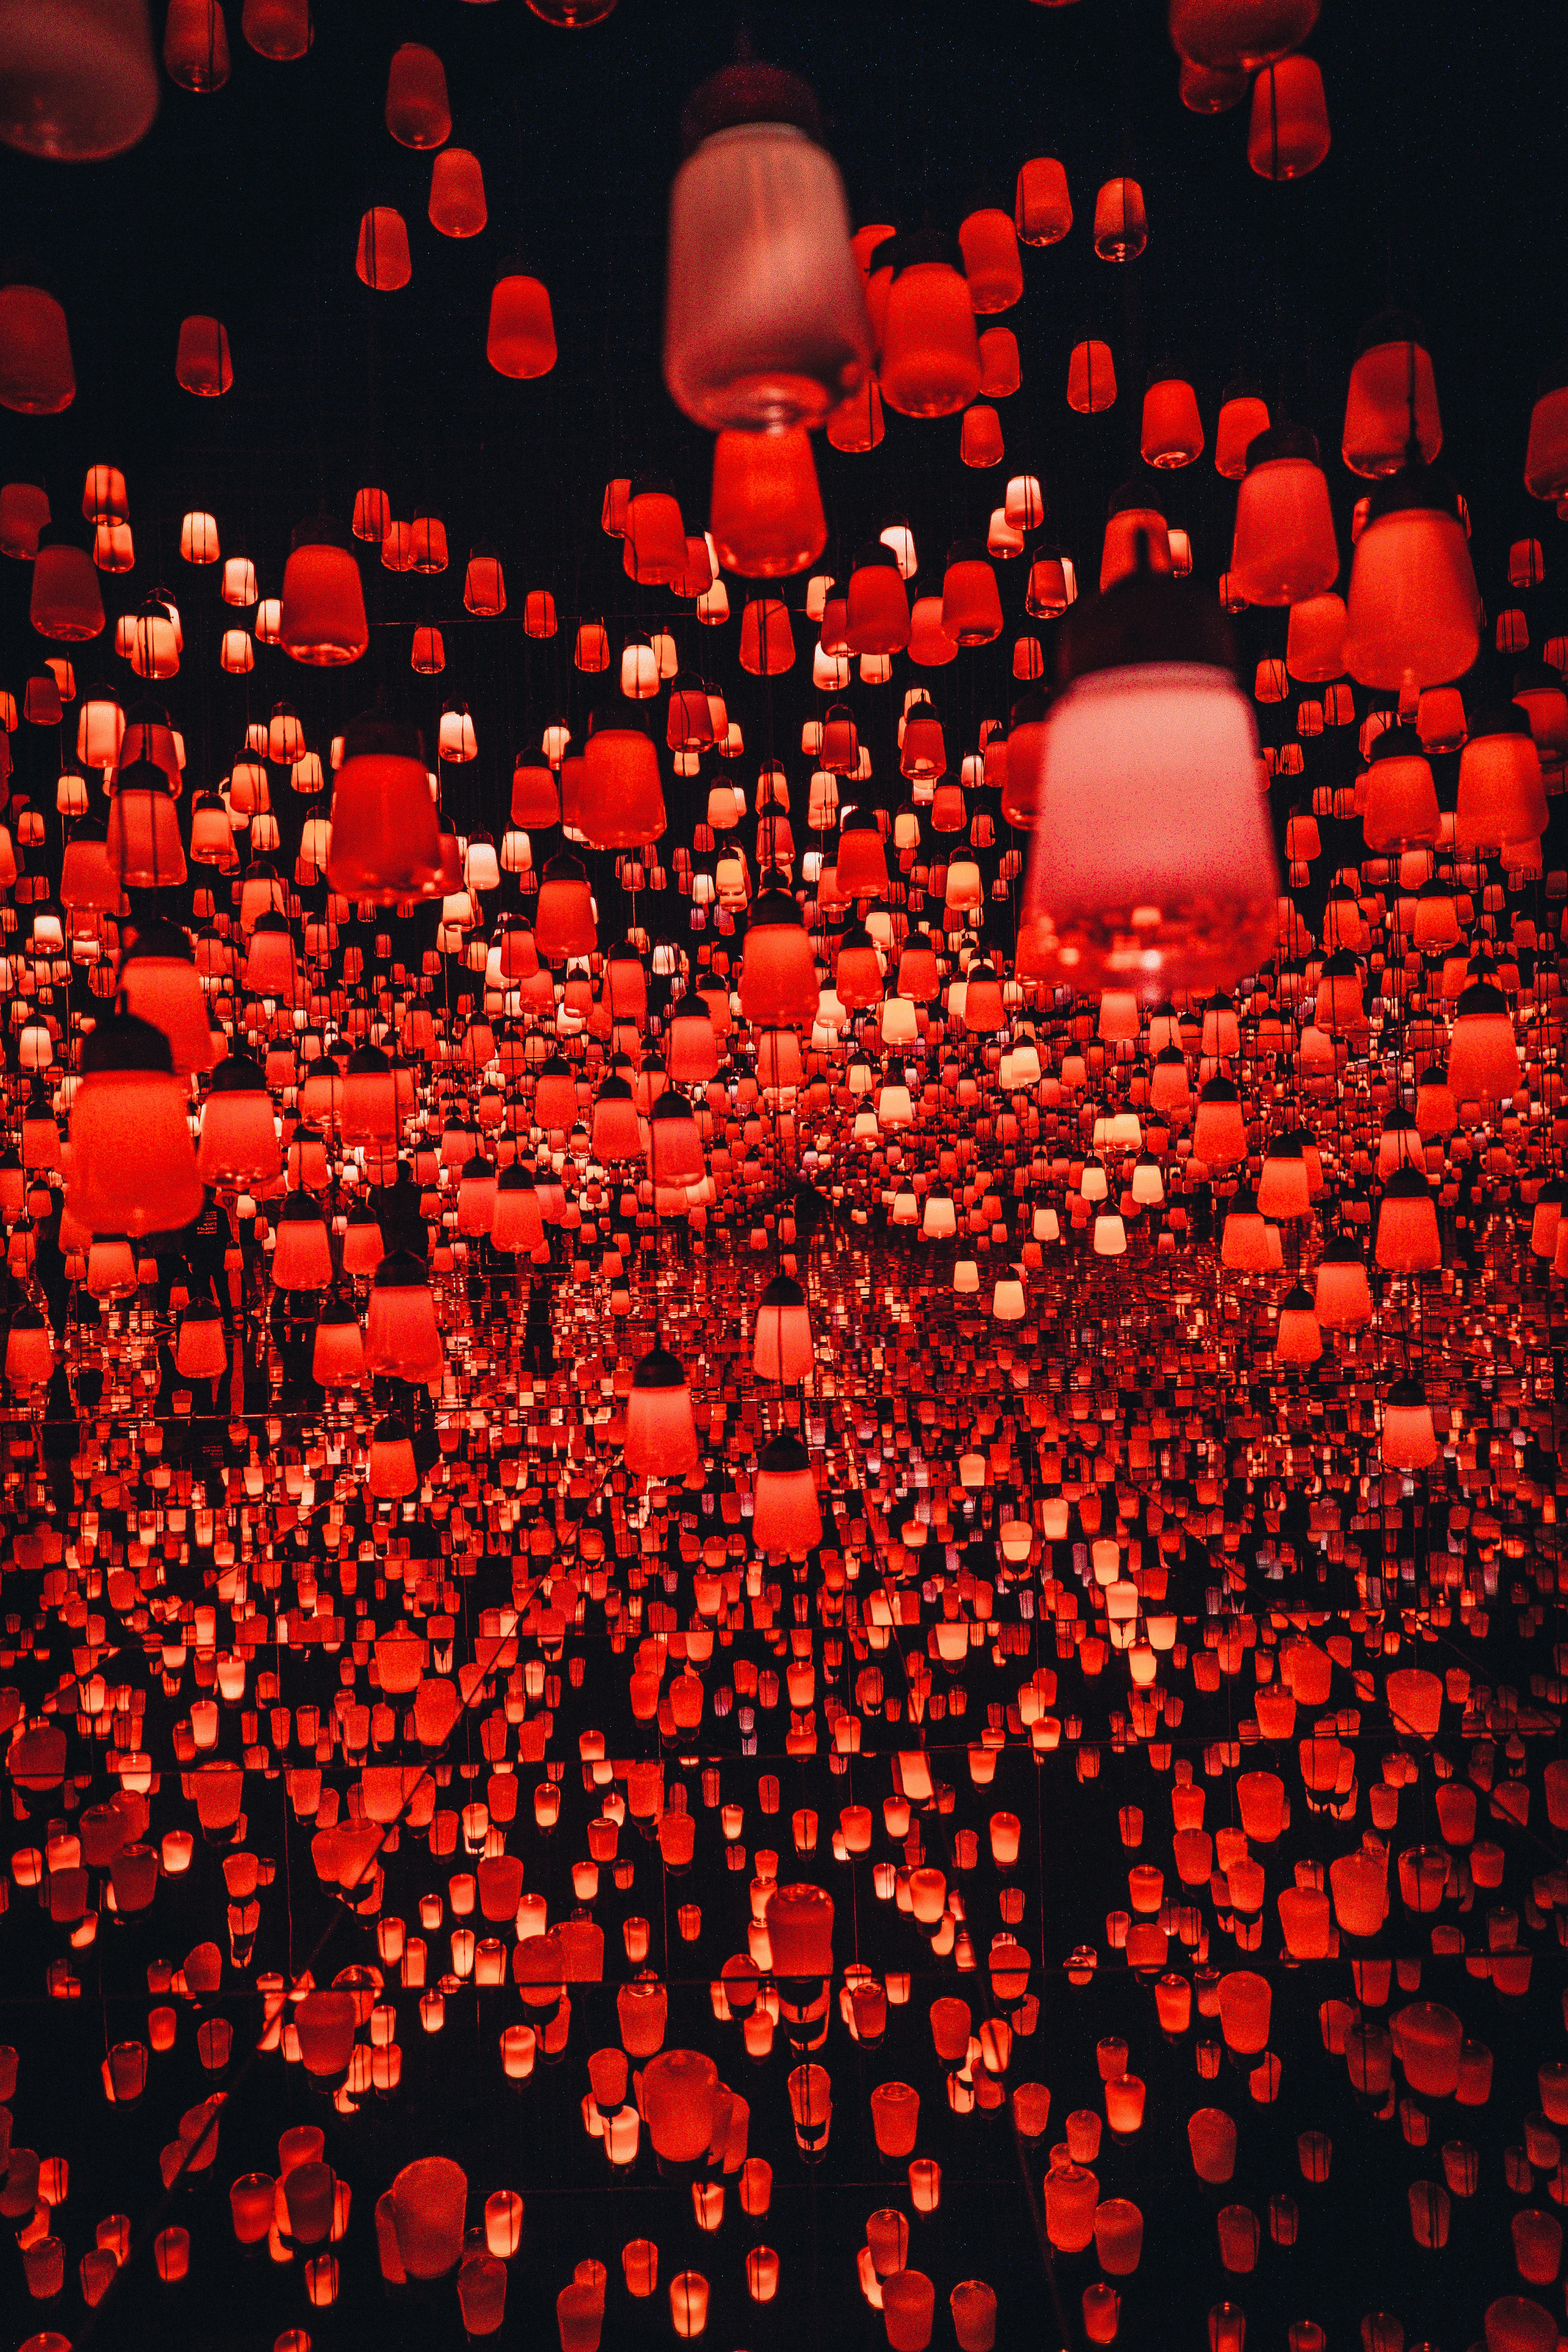
\includegraphics[width=6cm]{Figures/logo}}  %NEW: Changing logo
\def\extraspace{\vspace*{1.6cm}}
\makeatletter
\def\contactdetails{\faicon{phone} & \@telephone \\
                    \faicon{envelope} & \@email}
\makeatother

%%%% FRONT PAGE OF REPORTS

\def\reporttype{Report for}

\long\def\front#1#2#3{
\newpage
\begin{singlespacing}
\thispagestyle{empty}
\vspace*{-1.4cm}
\hspace*{-1.4cm}
\hbox to 16cm{
  \hbox to 6.5cm{\vbox to 14cm{\vbox to 25cm{
    \logo
    \vfill
    \parbox{6.3cm}{\raggedright
      \sf\color[rgb]{0.8, 0.7, 0.1 }    % NEW color 
      {\large\textbf{\name}}\par
      \vspace{.7cm}
      \tabcolsep=0.12cm\sf\small
      \begin{tabular}{@{}ll@{}}\contactdetails
      \end{tabular}
      \vspace*{0.3cm}\par
      ABN: \abn\par
    }
  }\vss}\hss}
  \hspace*{0.2cm}
  \hbox to 1cm{\vbox to 14cm{\rule{4pt}{26.8cm}\vss}\hss\hfill}  %NEW: Thicker line
  \hbox to 10cm{\vbox to 14cm{\vbox to 25cm{   
      \vspace*{3cm}\sf\raggedright
      \parbox{11cm}{\sf\raggedright\baselineskip=1.2cm
         \fontsize{24.88}{30}\color[rgb]{0, 0.29, 0.55}\sf\textbf{#1}}   % NEW: title color blue
      \par
      \vfill
      \large
      \vbox{\parskip=0.8cm #2}\par
      \vspace*{2cm}\par
      \reporttype\\[0.3cm]
      \hbox{#3}%\\[2cm]\
      \vspace*{1cm}
      {\large\sf\textbf{\Date~\Month~\Year}}
   }\vss}
  }}
\end{singlespacing}
\newpage
}

\makeatletter
\def\titlepage{\front{\expandafter{\@title}}{\@author}{\@organization}}
\makeatother

\usepackage{setspace}
\setstretch{1.5}

%% Any special functions or other packages can be loaded here.
\usepackage{booktabs}
\usepackage{longtable}
\usepackage{array}
\usepackage{multirow}
\usepackage{wrapfig}
\usepackage{float}
\usepackage{colortbl}
\usepackage{pdflscape}
\usepackage{tabu}
\usepackage{threeparttable}
\usepackage{threeparttablex}
\usepackage[normalem]{ulem}
\usepackage{makecell}
\usepackage{xcolor}


\begin{document}
\titlepage

{
\setcounter{tocdepth}{2}
\tableofcontents
}
\hypertarget{report-introduction}{%
\section{Report Introduction}\label{report-introduction}}

In this report, we are exploring the relationship between the three main pillars of CO2 emissions, Urban Population and Energy Usage produced carbon footprints. All of which we have chosen wide range of countries with different income level to explore further into more fruitful results that would answer our corresponding research questions. Countries are including but not limited to China, USA, Vietnam, Japan, Thailand and Uganda. Therefore, each own section in this report will be divided by countries used which has its own research questions along with figures and tables answering and analyzing its questions.

\hypertarget{section-1}{%
\section{Section 1}\label{section-1}}

\section*{Country China and USA}

\hypertarget{introduction}{%
\subsection{Introduction}\label{introduction}}

This section studies the relationship between per capita carbon dioxide emissions and urban population in China and the United States.

\hypertarget{research-question}{%
\subsection{Research question}\label{research-question}}

Q1:Changes in per capita carbon dioxide emissions per 15 years in China and the United States.

Q2:Is there a linear relationship between per capita CO2 emissions and urban population in the USA?

\hypertarget{exploratory-data-analysis}{%
\subsection{Exploratory data analysis}\label{exploratory-data-analysis}}

\begin{itemize}
\tightlist
\item
  Q1
\end{itemize}

\begin{table}[!h]

\caption{\label{tab:CO2tab}CO2 emissions per capita in China and USA per 15 years from 1960 to 2014}
\centering
\resizebox{\linewidth}{!}{
\begin{tabular}[t]{lrrrr}
\toprule
Country\_Name & emissons\_1960\_1969 & emissons\_1975\_1989 & emissons\_1990\_2004 & emissons\_2005\_2014\\
\midrule
\cellcolor{gray!6}{China} & \cellcolor{gray!6}{0.8317398} & \cellcolor{gray!6}{1.670062} & \cellcolor{gray!6}{2.763562} & \cellcolor{gray!6}{6.287833}\\
USA & 18.8078609 & 20.038491 & 19.509787 & 17.707995\\
\bottomrule
\end{tabular}}
\end{table}

In table \ref{tab:CO2tab}, I find that China's per capita CO2 emissions have been decreasing since 1960, while the US per capita CO2 emissions have also been decreasing after a small increase from 1977-1989.

\begin{itemize}
\tightlist
\item
  Q2
\end{itemize}

\begin{figure}[H]

{\centering \includegraphics{report_files/figure-latex/figure-1-1} 

}

\caption{Relationship between per capita CO2 emissions and urban population}\label{fig:figure-1}
\end{figure}

In figure \ref{fig:figure-1}, I found that there is not an significant linear relationship between per capita CO2 emissions and urban population in the USA.

\hypertarget{conclusion}{%
\subsection{Conclusion}\label{conclusion}}

\textcite{alam2016relationships} indicated that energy consumption and population growth are important factors in responding to economic development. The gradual reduction of CO2 emissions per capita in China and the USA is a reflection of the positive economic development of these countries. However, the correlation between per capita CO2 emissions and population growth in the USA is not shown in this section.

\hypertarget{section-2}{%
\section{Section 2}\label{section-2}}

\section*{Vietnam and Japan}

\hypertarget{introduction-1}{%
\subsection{Introduction}\label{introduction-1}}

In the section we will compare between Vietnam and Japan in terms of CO2 emissions, urban population and energy use.

\hypertarget{research-questions}{%
\subsection{Research questions}\label{research-questions}}

Q1: The urbanization rate between high income country and low-middle income country.

Q2: The relationship between the amount of CO2 emitted and the energy use per capital and comparison between two countries.

\hypertarget{exploratory-data-analysis-1}{%
\subsection{Exploratory data analysis}\label{exploratory-data-analysis-1}}

\begin{itemize}
\tightlist
\item
  Q1
\end{itemize}

\begin{table}[!h]

\caption{\label{tab:urban}Rate of urbanization between Japan and Vietnam over time}
\centering
\begin{tabular}[t]{lr}
\toprule
Country\_Name & average\_rate\\
\midrule
\cellcolor{gray!6}{Japan} & \cellcolor{gray!6}{0.979718}\\
Vietnam & 3.662266\\
\bottomrule
\end{tabular}
\end{table}

\textcite{8809066} revealed that almost 50\% of the world population now live in big cities.

Particularly, the rate of urban growth is seen to be higher in developing countries, in comparison to developed countries.

In table \ref{tab:urban} we can observe that urban growth in Vietnam is higher than in Japan from 1971 to 2013.

This may be due to the fact that for high income nations like Japan, urbanization has occurred earlier and majority of the country's population have already lived in big cities, whereas in low-middle countries like Vietnam, this process only started to happen in recent decades.

\begin{itemize}
\tightlist
\item
  Q2
\end{itemize}

\begin{figure}

{\centering \includegraphics[width=0.7\linewidth]{Figures/CO2emissions-1} 

}

\caption{Relationship between the energy use and CO2 emissions in Japan and Vietnam}\label{fig:CO2emissions}
\end{figure}

Energy consumption has been considered one of the biggest contributor to the increase of CO2 emissions around the world. According to \textcite{WANG20182144}, energy consumption worldwide has grew by 2.3\%, associated with an increase of 1.7\% Co2 emissions into the atmosphere.

Moreover, \textcite{owidenergy} demonstrated that there are huge inequalities in energy consumption between developed and developing countries.

Figure \ref{fig:CO2emissions} indicates a positive correlation between the amount of energy consumption and CO2 emission. Noticeably, Japan has showed a sharper increase in the energy consumption than Vietnam over the years.

\hypertarget{conclusion-1}{%
\subsection{Conclusion}\label{conclusion-1}}

Regarding the urbanization rate among countries, it is obvious that the urban growth in Japan happened more slowly than in Vietnam.

Regarding the energy use and CO2 emission, it can be seen that there was a overall increase in energy consumption and CO2 emission in both countries over the years. However, the amount of CO2 emission in Japan was much higher than in Vietnam, in response to larger consumption of energy in the country.

\hypertarget{section-3}{%
\section{Section 3}\label{section-3}}

\section*{Thailand and Uganda}

\hypertarget{introduction-2}{%
\subsection{Introduction}\label{introduction-2}}

As the general world trend is increasingly rely on heavy energy consumption, most notably fossil fuels, in order to catch up with the ever-growing number of population, the unfortunate and unwanted by-pass product of processing petrol and energy in form of CO2 is increasing rapidly as well. In this section, we are looking at Thailand and Uganda trends for CO2 - representatives for developing countries wit the following research questions:

\hypertarget{research-questions-1}{%
\subsection{Research questions}\label{research-questions-1}}

\begin{itemize}
\tightlist
\item
  1st Research Question, between the two selected countries, what are relationship between CO2 emissions and Urban Population that cause its visible trends of increasing/decreasing/sideways nature? (Given the absent of Energy Use of Oil data variable in Uganda and Data availability of CO2 Emission up to 2014)
\item
  2nd Research Question, what is the average 1960-2010 trend for both country regarding their CO2 emissions?
\end{itemize}

\hypertarget{exploratory-data-analysis-2}{%
\subsection{Exploratory data analysis}\label{exploratory-data-analysis-2}}

\begin{itemize}
\tightlist
\item
  Q1
\end{itemize}

As we are looking at the trend for CO2 emission in figure\ref{fig:figure1}) for both countries, it is clear that Thailand has significantly sharp incline trend while Uganda has a surprisingly stable and sideways trend in comparison. In this instance, it can be assure that not all countries that are labelled ``Developing Country'' would have similar trends of CO2 emission on the superficial level.

\begin{figure}[H]

{\centering \includegraphics[width=0.7\linewidth]{report_files/figure-latex/figure1-1} 

}

\caption{CO2 Emission Trend}\label{fig:figure1}
\end{figure}

\begin{itemize}
\tightlist
\item
  Q2
\end{itemize}

As for the second question, referring to table\ref{tab:table1}), we can see that the average of CO2 emissions from both countries are significantly different from the span of 1960-2010. Thus far, it can be implied that, not every country, regardless of ``developing country'' needs to have the incline trend of CO2 emission per capita.

\begin{table}[!h]

\caption{\label{tab:table1}Average CO2 Emissions from 1960-2010}
\centering
\begin{tabular}[t]{lrlr}
\toprule
Country...1 & average\_CO2\_Emission...2 & Country...3 & average\_CO2\_Emission...4\\
\midrule
\cellcolor{gray!6}{Thailand} & \cellcolor{gray!6}{1.616342} & \cellcolor{gray!6}{Uganda} & \cellcolor{gray!6}{0.072436}\\
\bottomrule
\end{tabular}
\end{table}

\hypertarget{conclusion-2}{%
\subsection{Conclusion}\label{conclusion-2}}

In conclusion, we can simply understand that the general trend of CO2 emissions that most people assume would be increasing constantly year to year would be applied to all countries around the world is mistakenly understood. In the reality is that every country has their own CO2 emissions trend (can even be sideways or decreasing) which totally depends on factors that are not listed in this data set. Especially in Uganda, \textcite{waaswa2020development} point that agricultural activities (e.g.~synthetic fertilizer) contribute a prominent number of emission to overall CO2. Therefore, number must not be imply superficially but must be with specific and suitable data.

\hypertarget{report-conclusion}{%
\section{Report Conclusion}\label{report-conclusion}}

With all research questions explored and answered, CO2 emission is a harmful cause which most countries are experiencing. Regardless of how much emissions they produce, every nation must try to minimize CO2 emissions and its increasing trend for the better future.

\printbibliography

\end{document}
